\subsection{Calibration}
\label{sec:calibration}
In order to calibrate the detector the pulse generator was used to injected in
the pre-amplifier a known pulse. The oscilloscope was used to read the pulse
voltage that multiplied by the pre-amplifier capacitance gives the collected
charge as described in Section~\ref{sec:meas-appar}. The distribution on the MCA
was fitted with a Gaussian using the data taking software, the mean value is
then associated to a charge and the standard deviation used as uncertainty. This
procedure was performed for a set of input voltages and, due to time
restrictions, only for a gain value of 100. Figure~\ref{fig:calibration_fit}
shows the calculated collected charge as a function of the MCA channel number
with a linear fit superimposed. Figure~\ref{fig:calibration_raw} shows the
counts as a function of the MCA channel number.
\begin{figure}[!h]
  \centering
  \begin{subfigure}[t]{.48\linewidth}
    \includegraphics[width=\linewidth]{calibration_fit}
    \caption{Collected charge as a function of the multi-channel number}
    \label{fig:calibration_fit}
  \end{subfigure}
  \begin{subfigure}[t]{.48\linewidth}
    \includegraphics[width=\linewidth]{calibration_raw}
    \caption{Counts as a function of the multi-channel number}
    \label{fig:calibration_raw}
  \end{subfigure}
  \caption{}
  \label{fig:calibration}
\end{figure}

\subsection{Errors}


The relationship between the HV:

\begin{equation}
  U_{HV(U_{ref})} = \alpha U_{ref} + \beta
\end{equation}

from where we can get the error as:

\begin{equation}
  \delta U_{HV(U_{ref})} = \sqrt{ (\delta \alpha  U_{ref})^2 + (\delta \beta)^2 + (\alpha \delta U_{ref})^2 }
\end{equation}

The charge collected in the anode was obtained feeding the input of the preamplifier with a square pulse and measuring the MCA response.

\begin{equation}
  Q = C U_{pulse (N)} 
\end{equation}

Where Q is the charge collected, the C capacitance and N is the multichannel analyzer response that depends lineary on the gain chosen.

\begin{equation}
  U_{pulse (N)}= C\alpha_G N_G + \beta_G
\end{equation}

Hence the error for Q would be:

\begin{equation}
  \delta Q = \sqrt{(\delta CU_p )^2 + (C \sqrt{(N\delta \alpha)^2+(\delta \beta)^2} )^2 + (C\alpha \delta N)^2}
\end{equation}

On the resolution side most errors treated and obtained from the Gaussian distribution

\begin{equation}
  \delta R = \sqrt{(\frac{\delta \sigma,}{\sigma})^2 + (\frac{\delta \mu}{\mu})^2}
\end{equation}



\begin{figure}[!h]
  \centering
  \begin{subfigure}[t]{.48\linewidth}
    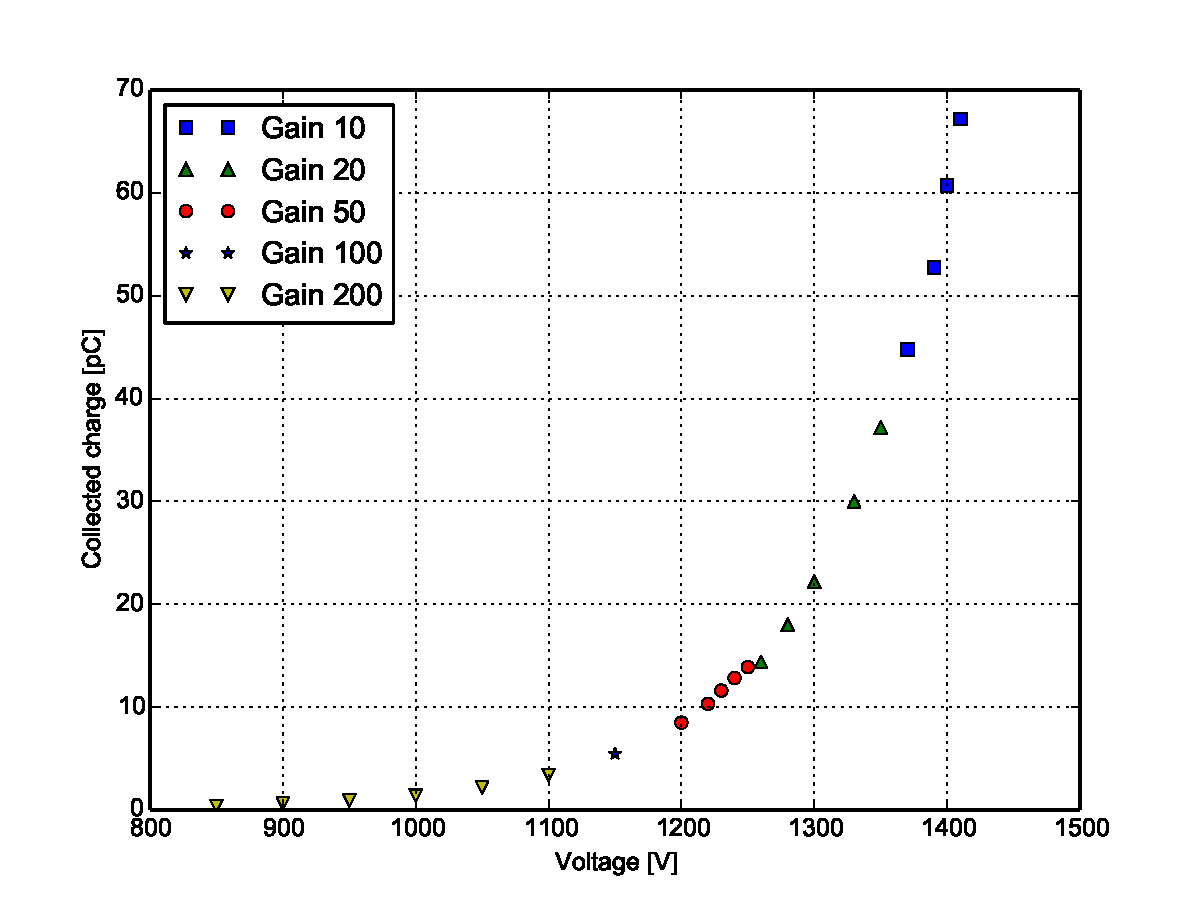
\includegraphics[width=\linewidth]{charge_vs_voltage}
    \caption{}
    \label{fig:charge_vs_voltage}
  \end{subfigure}
  \begin{subfigure}[t]{.48\linewidth}
    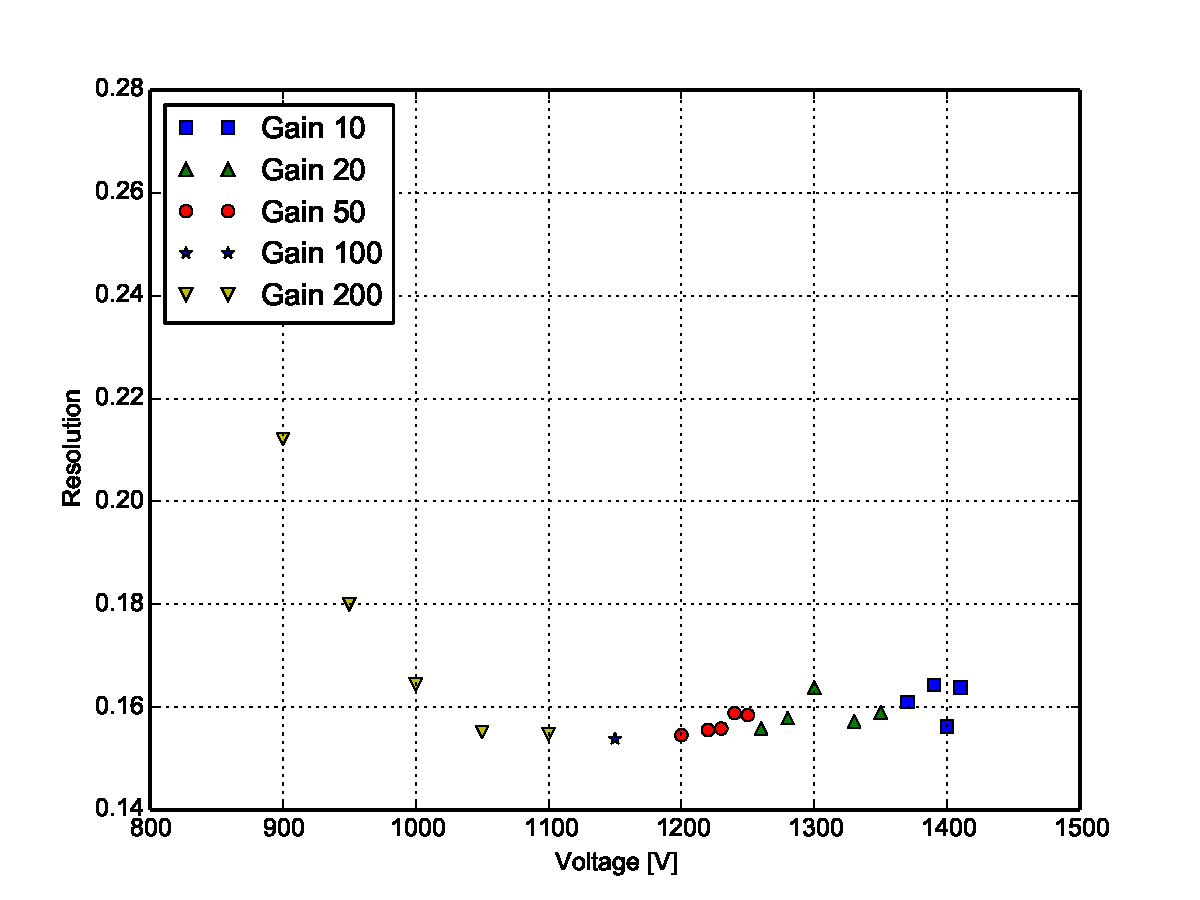
\includegraphics[width=\linewidth]{resolution_vs_voltage}
    \caption{}
    \label{fig:resolution_vs_voltage}
  \end{subfigure}
  \caption{}
  \label{fig:results}
\end{figure}

%%% Local Variables:
%%% mode: latex
%%% TeX-master: "prop_counter"
%%% End:
